\documentclass[12pt]{article}
\usepackage{amsmath}
\usepackage{graphicx}
\begin{document}
\providecommand{\pr}[1]{\ensuremath{\Pr\left(#1\right)}}
\providecommand{\prt}[2]{\ensuremath{p_{#1}^{\left(#2\right)} }}        % own macro for this question
\providecommand{\qfunc}[1]{\ensuremath{Q\left(#1\right)}}
\providecommand{\sbrak}[1]{\ensuremath{{}\left[#1\right]}}
\providecommand{\lsbrak}[1]{\ensuremath{{}\left[#1\right.}}
\providecommand{\rsbrak}[1]{\ensuremath{{}\left.#1\right]}}
\providecommand{\brak}[1]{\ensuremath{\left(#1\right)}}
\providecommand{\lbrak}[1]{\ensuremath{\left(#1\right.}}
\providecommand{\rbrak}[1]{\ensuremath{\left.#1\right)}}
\providecommand{\cbrak}[1]{\ensuremath{\left\{#1\right\}}}
\providecommand{\lcbrak}[1]{\ensuremath{\left\{#1\right.}}
\providecommand{\rcbrak}[1]{\ensuremath{\left.#1\right\}}}
\newcommand{\sgn}{\mathop{\mathrm{sgn}}}
\providecommand{\abs}[1]{\left\vert#1\right\vert}
\providecommand{\res}[1]{\Res\displaylimits_{#1}} 
\providecommand{\norm}[1]{\left\lVert#1\right\rVert}
%\providecommand{\norm}[1]{\lVert#1\rVert}
\providecommand{\mtx}[1]{\mathbf{#1}}
\providecommand{\mean}[1]{E\left[ #1 \right]}
\providecommand{\cond}[2]{#1\middle|#2}
\providecommand{\fourier}{\overset{\mathcal{F}}{ \rightleftharpoons}}
\newenvironment{amatrix}[1]{%
  \left(\begin{array}{@{}*{#1}{c}|c@{}}
}{%
  \end{array}\right)
}
%\providecommand{\hilbert}{\overset{\mathcal{H}}{ \rightleftharpoons}}
%\providecommand{\system}{\overset{\mathcal{H}}{ \longleftrightarrow}}
	%\newcommand{\solution}[2]{\textbf{Solution:}{#1}}
\newcommand{\solution}{\noindent \textbf{Solution: }}
\newcommand{\cosec}{\,\text{cosec}\,}
\providecommand{\dec}[2]{\ensuremath{\overset{#1}{\underset{#2}{\gtrless}}}}
\newcommand{\myvec}[1]{\ensuremath{\begin{pmatrix}#1\end{pmatrix}}}
\newcommand{\mydet}[1]{\ensuremath{\begin{vmatrix}#1\end{vmatrix}}}
\newcommand{\myaugvec}[2]{\ensuremath{\begin{amatrix}{#1}#2\end{amatrix}}}
\providecommand{\rank}{\text{rank}}
\providecommand{\pr}[1]{\ensuremath{\Pr\left(#1\right)}}
\providecommand{\qfunc}[1]{\ensuremath{Q\left(#1\right)}}
	\newcommand*{\permcomb}[4][0mu]{{{}^{#3}\mkern#1#2_{#4}}}
\newcommand*{\perm}[1][-3mu]{\permcomb[#1]{P}}
\newcommand*{\comb}[1][-1mu]{\permcomb[#1]{C}}
\providecommand{\qfunc}[1]{\ensuremath{Q\left(#1\right)}}
\providecommand{\gauss}[2]{\mathcal{N}\ensuremath{\left(#1,#2\right)}}
\providecommand{\diff}[2]{\ensuremath{\frac{d{#1}}{d{#2}}}}
\providecommand{\myceil}[1]{\left \lceil #1 \right \rceil }
\newcommand\figref{Fig.~\ref}
\newcommand\tabref{Table~\ref}
\newcommand{\sinc}{\,\text{sinc}\,}
\newcommand{\rect}{\,\text{rect}\,}
%%
%	%\newcommand{\solution}[2]{\textbf{Solution:}{#1}}
%\newcommand{\solution}{\noindent \textbf{Solution: }}
%\newcommand{\cosec}{\,\text{cosec}\,}
%\numberwithin{equation}{section}
%\numberwithin{equation}{subsection}
%\numberwithin{problem}{section}
%\numberwithin{definition}{section}
%\makeatletter
%\@addtoreset{figure}{problem}
%\makeatother

%\let\StandardTheFigure\thefigure
\let\vec\mathbf

Question 1.3.3 $D_{1}$ is a point on BC such that
$AD_{1}\perp BC$and $AD_{1} $ is defined to be the altitude.
Find the equations of the altitude $BE_{1} $ and $CF_{1}$
to the sides AC and AB respectively.

  
{Solution}:
Let 
\begin{align}\vec{A}=\myvec{1\\-1\\}
\vec{B}=\myvec{-4 \\6 \\}
\vec{C}=\myvec{-3\\-5\\}
\end{align}
Directional vector of $AB=\vec{B}-\vec{A}$
\begin{align}
\vec{m}_{AB}=\myvec{-4\\6\\}
-\myvec{1\\-1 \\}
=\myvec{-5\\7\\}
\end{align}
Similarly,
Directional vector of $AC=\vec{C}-\vec{A}$
\begin{align}
\vec{m}_{AC}=\myvec{-3\\-5\\}
-\myvec{1\\-1\\}
=\myvec{-4\\-4\\}
\end{align}
Directional vectors perpendicular to AB and AC
\begin{align}
\vec{n}_{AC}=\vec{m}_{BE}=\myvec{4\\-4}
\end{align}
\begin{align}
\vec{n} &= \myvec{0&1 \\ -1&0}\vec{m}\\
&= \myvec{0&1 \\ -1&0}\myvec{4 \\ -4}\\
&= \myvec{-4 \\ -4}
\end{align}
\begin{align}
\vec{n}_{AB}=\vec{m}_{CF}=\myvec{7\\5}
\end{align}
\begin{align}
\vec{n} &= \myvec{0&1 \\ -1&0}\vec{m}\\
&= \myvec{0&1 \\ -1&0}\myvec{7 \\ 5}\\
&= \myvec{5 \\ -7}
\end{align}
The equation of a line can be represented by:
\begin{align}
\vec{n}^{T}(\vec{x}-\vec{p})=0
\end{align}
Therefore, the equation of line BE
\begin{align}
\myvec{-4&-4}(\vec{x}-\myvec{-4\\6\\})=0
\end{align}
Therefore, the equation of line CF
\begin{align}
\myvec{5&-7}(\vec{x}-\myvec{-3\\-5\\})=0
\end{align}
\begin{figure} [htbp]
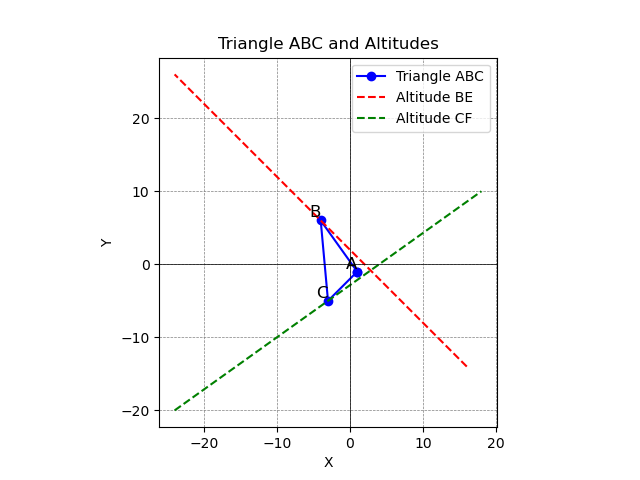
\includegraphics{/home/meena/Figs/figure.png}
\caption{Triangle ABC with altitudes BE and CF}
\label{fig}
\end{figure}
\end{document}
